We present results in five parts: cohort characterization, single-cell marker discovery, strict external validation, modality ablation, and external risk stratification.

\subsection{Cohort Characterization}

Table~\ref{tab:cohort} summarizes the cohorts used in the v7 study design. The CPTAC cohort provides the multimodal discovery resource, while TCGA serves as a held-out external test set. Fig.~\ref{fig:upset_modalities} shows that RNA+methylation is the dominant CPTAC intersection and that only 17 cases currently support full three-way transfer from bulk RNA, methylation, and scRNA.

\begin{table}[h]
\centering
\caption{Cohort summary for the v7 GBM benchmark.}
\label{tab:cohort}
\begin{tabular}{lr}
\toprule
Quantity & Value \\
\midrule
CPTAC training cases (RNA+clinical) & 195 \\
TCGA external test cases & 286 \\
CPTAC cases with RNA+methylation & 192 \\
scRNA source cases & 17 \\
Selected shared RNA genes & 256 \\
Transferred marker programs & 6 \\
1-year eligible cases (train/test) & 181 / 252 \\
3-year eligible cases (train/test) & 159 / 234 \\
\bottomrule
\end{tabular}
\end{table}

\begin{figure}[t]
\centering
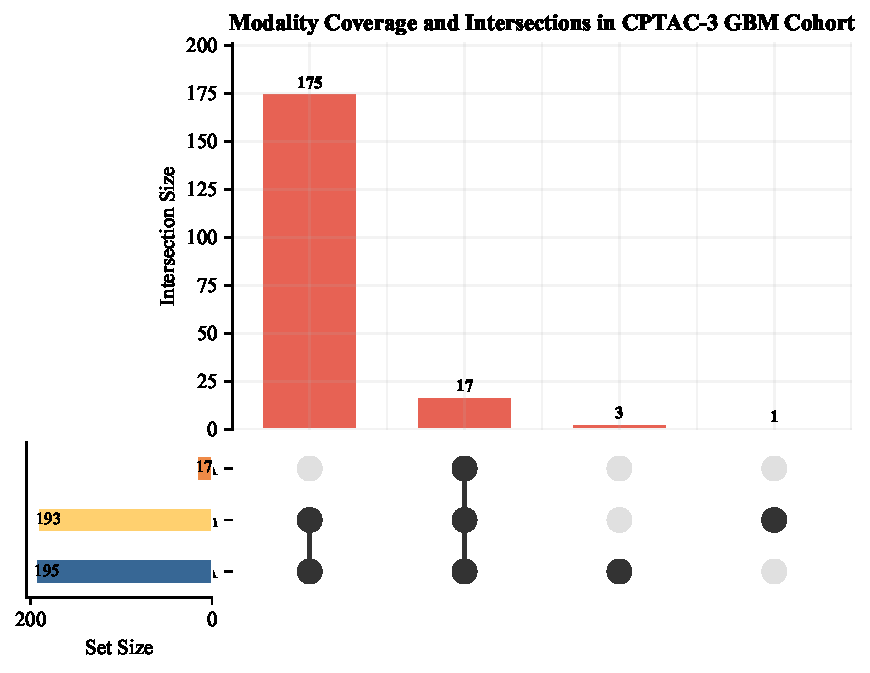
\includegraphics[width=0.48\textwidth]{figures/fig_upset_modalities.pdf}
\caption{UpSet plot showing modality coverage across 196 CPTAC-3 GBM cases. The dominant intersection is RNA+methylation, while only 17 cases support full RNA+methylation+scRNA transfer.}
\label{fig:upset_modalities}
\end{figure}

Fig.~\ref{fig:pca_tumor} projects the 192 CPTAC cases with matched RNA and methylation data into the first two principal components. Short-survival cases show partial separation, indicating that the multimodal feature space contains prognostic structure before any supervised modeling.

\begin{figure}[t]
\centering
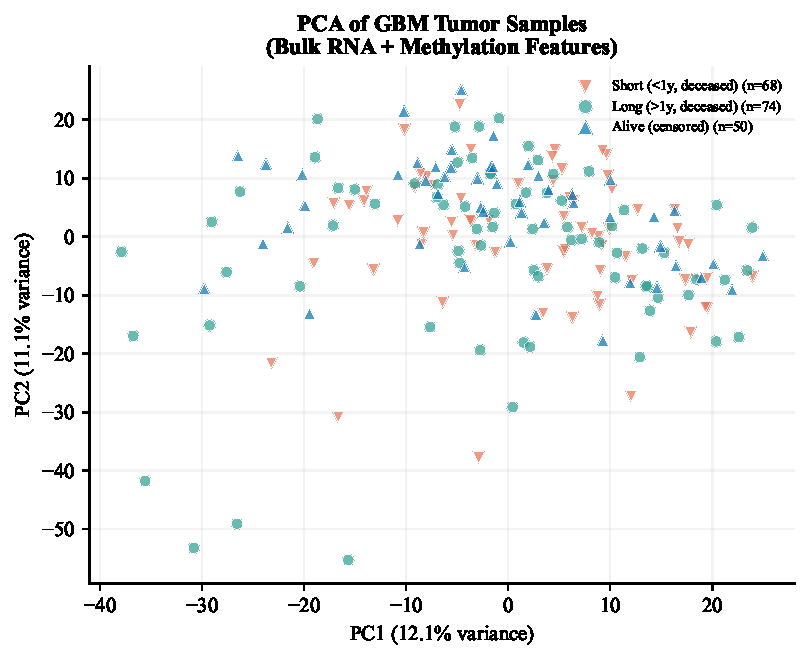
\includegraphics[width=0.48\textwidth]{figures/fig_pca_tumor.pdf}
\caption{PCA of 192 CPTAC GBM tumor samples using combined bulk RNA and methylation features. Samples are colored by survival group: short-survival deceased ($<1$ year), long-survival deceased ($\geq 1$ year), and alive (censored).}
\label{fig:pca_tumor}
\end{figure}

\subsection{Single-Cell Marker Discovery}

Fig.~\ref{fig:scrna_atlas} displays the cohort-level single-cell atlas from 17 GBM Seurat analysis outputs. Each panel shows case-specific UMAP embeddings colored by cluster assignment, revealing heterogeneous cellular compositions across patients.

\begin{figure*}[t]
\centering
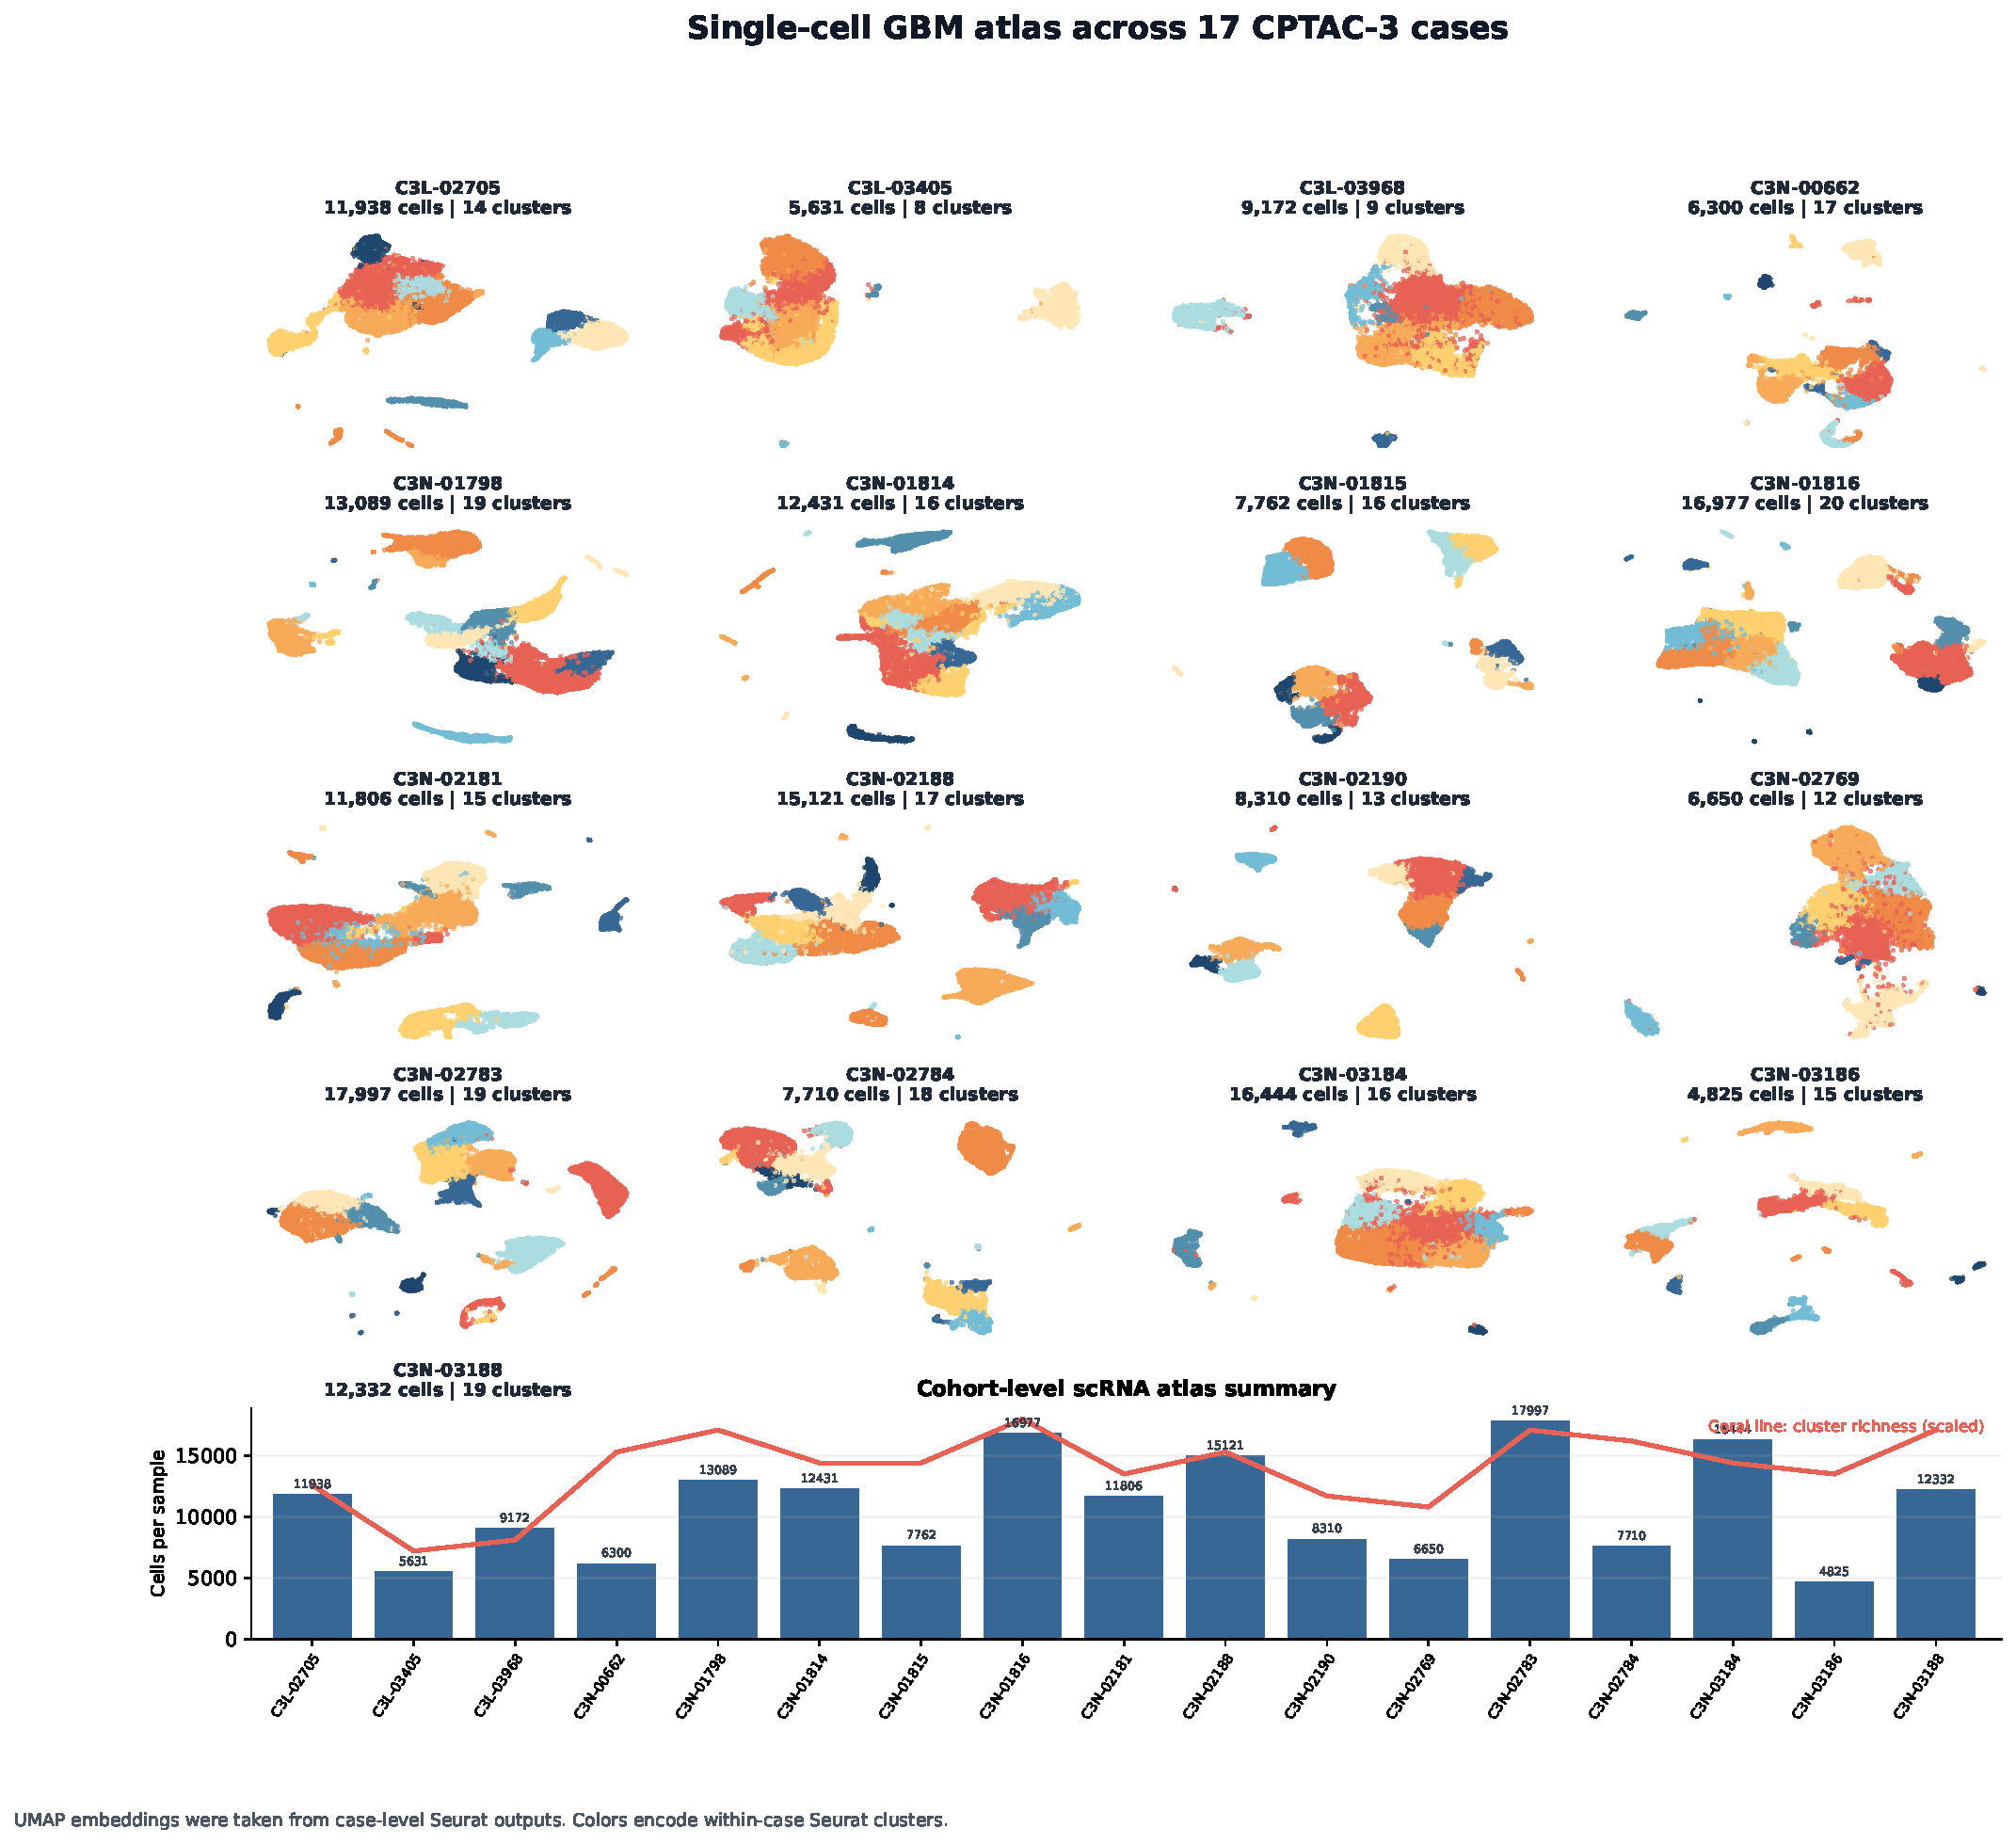
\includegraphics[width=0.95\textwidth]{figures/fig_scrna_atlas}
\caption{Cohort-level single-cell atlas from 17 GBM cases. Each panel shows case-specific UMAP embedding colored by Seurat cluster assignment, with a summary strip reporting total cells and cluster richness per case.}
\label{fig:scrna_atlas}
\end{figure*}

Fig.~\ref{fig:violin_celltypes} presents violin plots of cell-type proportions across the 17 scRNA-seq samples. Malignant subpopulations dominate, but immune and oligodendrocyte populations vary strongly between patients, motivating the use of soft transfer priors rather than hard cell-type labels.

\begin{figure*}[t]
\centering
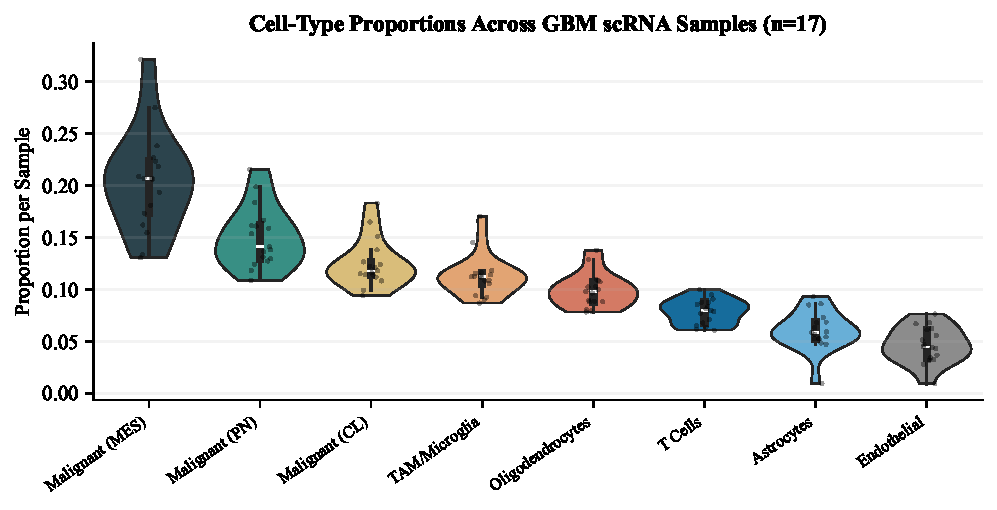
\includegraphics[width=0.92\textwidth]{figures/fig_violin_celltypes.pdf}
\caption{Violin plot of cell-type proportions across 17 GBM scRNA-seq samples. Each point represents one patient sample. Proportions were derived from Seurat cluster assignments with putative cell-type annotation.}
\label{fig:violin_celltypes}
\end{figure*}

Fig.~\ref{fig:volcano} shows the aggregated DEG landscape across all scRNA samples. A total of 610 genes are significantly upregulated and form the candidate pool from which the six transferred marker programs are derived.

\begin{figure}[t]
\centering
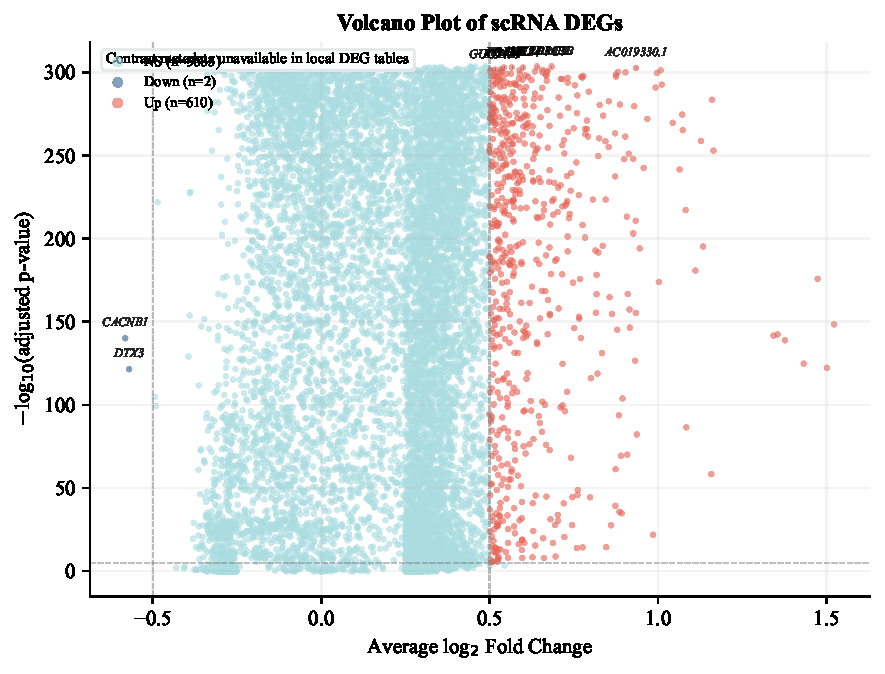
\includegraphics[width=0.48\textwidth]{figures/fig_volcano.pdf}
\caption{Volcano plot of DEGs from GBM scRNA-seq data. Upregulated (red, $n=610$) and downregulated (blue) genes are highlighted. Top genes are labeled. Thresholds: $|$log$_2$FC$| > 0.5$, $-$log$_{10}$(adj-$p$) $> 5$.}
\label{fig:volcano}
\end{figure}

Fig.~\ref{fig:dotplot_markers} confirms cluster-specific marker programs, and Fig.~\ref{fig:marker_heatmap} highlights the strongest recurrent markers across cases, including \textit{NKAIN2}, \textit{CNTNAP2}, \textit{ST18}, \textit{RNF220}, and \textit{NRG3}. These recurrent markers serve as the biological basis for the prior mask used by the proposed transformer.

\begin{figure*}[t]
\centering
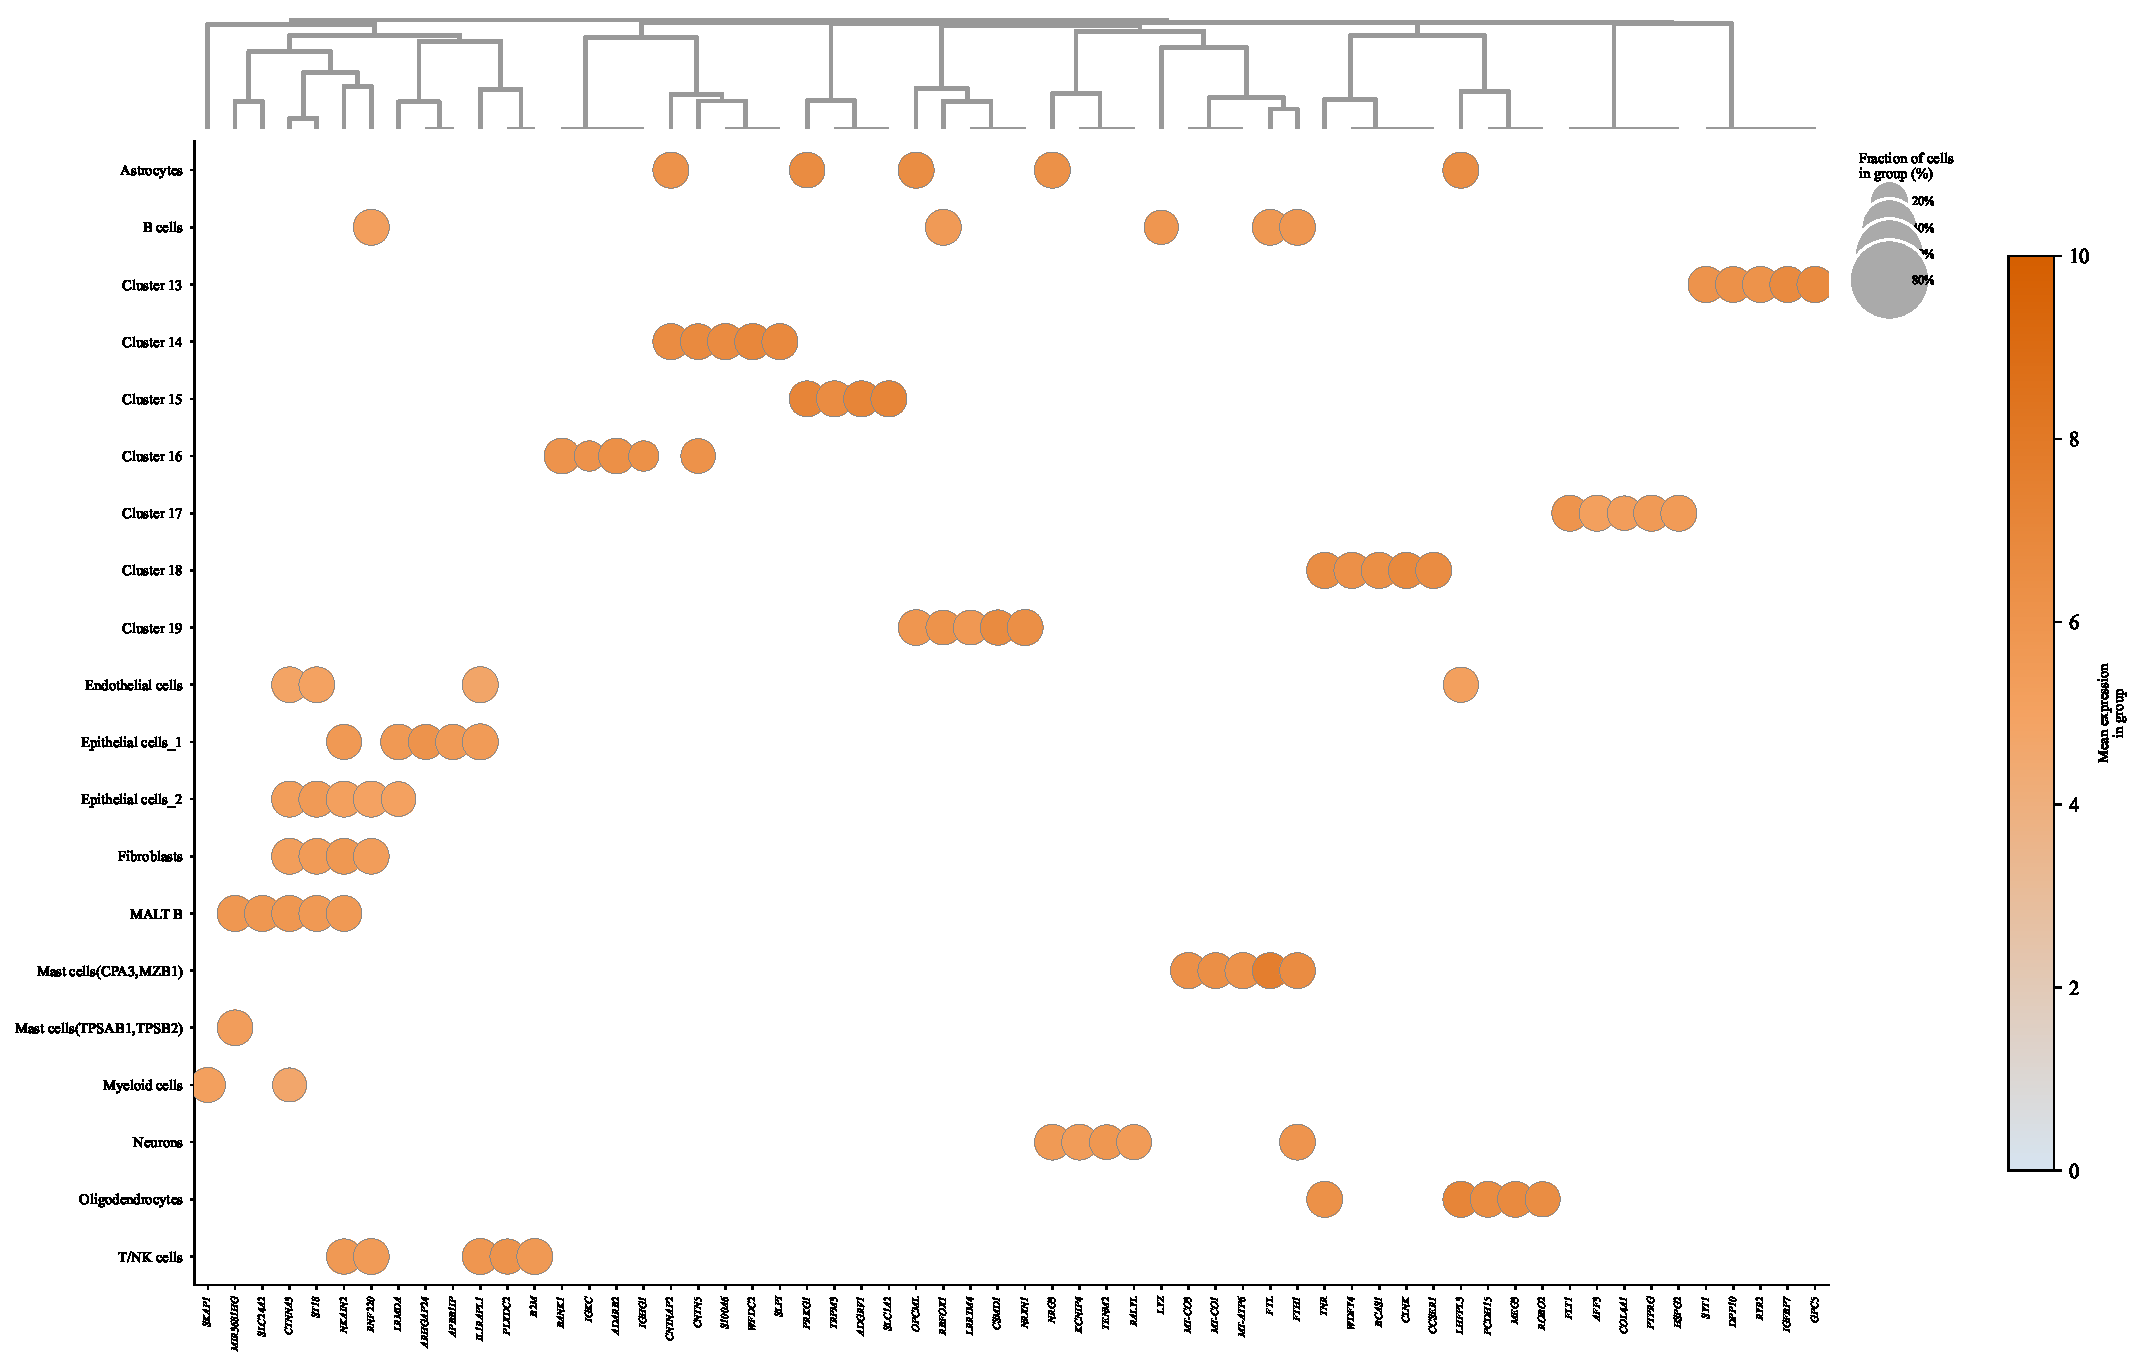
\includegraphics[width=0.95\textwidth]{figures/fig_dotplot_markers.pdf}
\caption{Dot plot of top marker genes across Seurat clusters from the 17 GBM scRNA samples. Dot size represents the proportion of cells expressing each gene in each cluster; color represents the average log$_2$ fold-change.}
\label{fig:dotplot_markers}
\end{figure*}

\begin{figure*}[t]
\centering
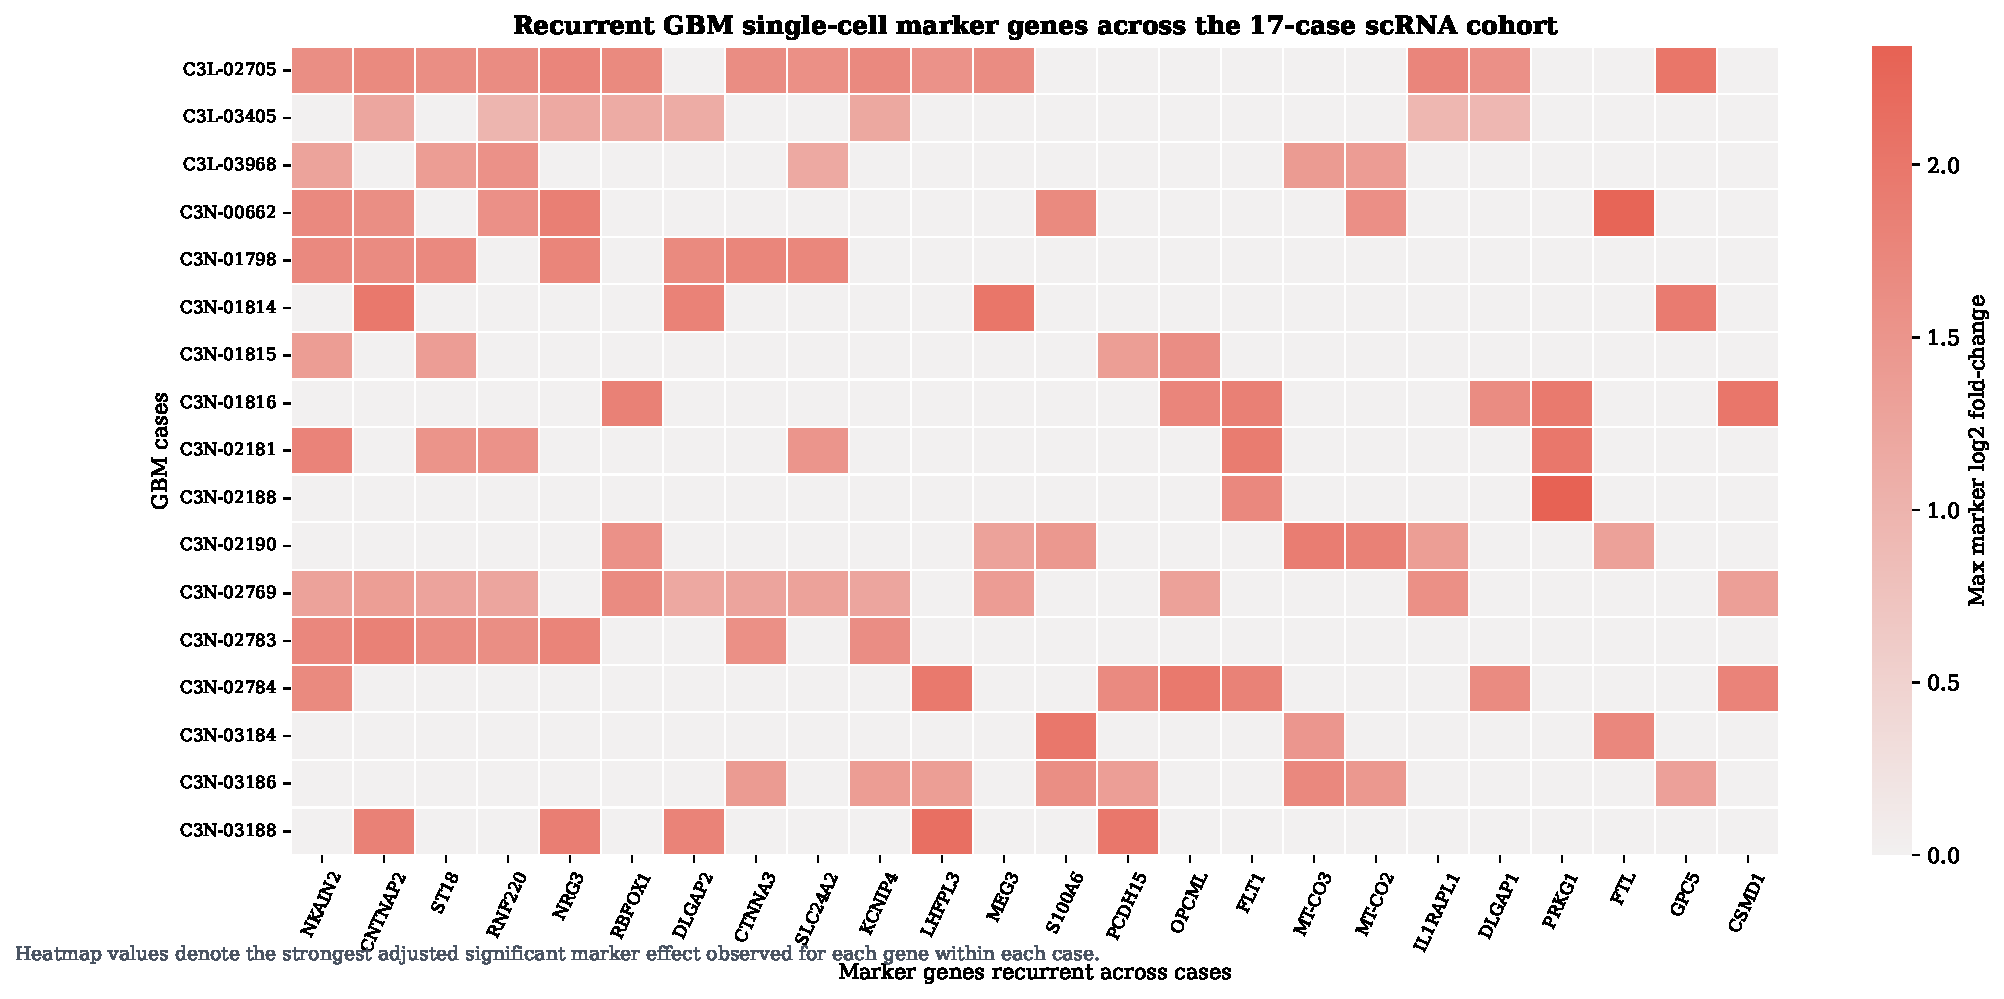
\includegraphics[width=0.95\textwidth]{figures/fig_marker_heatmap.pdf}
\caption{Heatmap of recurrent GBM marker genes across 17 scRNA cases. Genes are ranked by cross-case recurrence and strongest adjusted log$_2$ fold-change.}
\label{fig:marker_heatmap}
\end{figure*}

\subsection{Strict External Validation}

Table~\ref{tab:external_benchmark} reports the strict CPTAC$\rightarrow$TCGA benchmark. On the 1-year task, the compact transformer achieved the strongest external discrimination (AUC $=0.581$, C-index $=0.553$). On the 3-year task, LASSO logistic regression achieved the best AUC ($0.612$), while plain logistic regression achieved the best C-index ($0.586$). The prior-guided kernel transformer did not dominate the benchmark but remained competitive at the 3-year horizon (AUC $=0.586$), indicating that the prior mechanism is more promising for longer-horizon ranking than for short-horizon classification.

\begin{table*}[t]
\centering
\caption{Strict CPTAC$\rightarrow$TCGA external validation results.}
\label{tab:external_benchmark}
\begin{tabular}{lcccc}
\toprule
Model & 1-Year AUC & 1-Year C-index & 3-Year AUC & 3-Year C-index \\
\midrule
Logistic Regression & 0.548 & 0.540 & 0.592 & \textbf{0.586} \\
LASSO Logistic & 0.550 & 0.533 & \textbf{0.612} & 0.558 \\
Ridge Regression & 0.474 & 0.494 & 0.565 & 0.563 \\
SVM (RBF) & 0.506 & 0.512 & 0.502 & 0.546 \\
Random Forest & 0.538 & 0.531 & 0.539 & 0.569 \\
Gradient Boosting & 0.519 & 0.519 & 0.546 & 0.542 \\
SNN & 0.544 & 0.529 & 0.504 & 0.526 \\
Compact Transformer & \textbf{0.581} & \textbf{0.553} & 0.599 & 0.544 \\
Prior-Guided Kernel Transformer + SVM & 0.516 & 0.498 & 0.586 & 0.542 \\
\bottomrule
\end{tabular}
\end{table*}

Fig.~\ref{fig:v7_external_roc} shows the external ROC curves for all models. The overlap among classical and deep curves reinforces a central empirical point of this study: under strict external validation, GBM prognosis has a relatively low but stable discrimination ceiling, and architectural complexity alone does not guarantee better generalization.

\begin{figure*}[t]
\centering
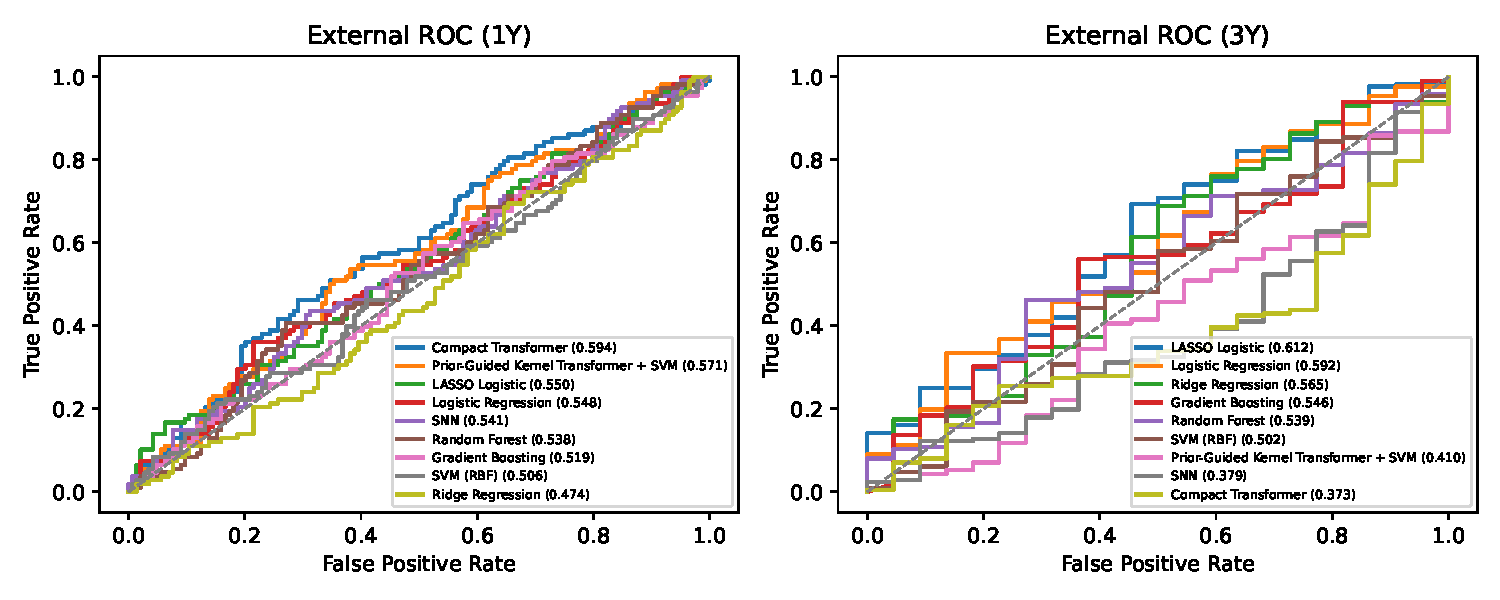
\includegraphics[width=0.95\textwidth]{figures/fig_v7_external_roc.pdf}
\caption{External ROC curves on TCGA for all v7 models. Left: 1-year endpoint. Right: 3-year endpoint. The compact transformer leads at 1 year, while LASSO logistic leads at 3 years.}
\label{fig:v7_external_roc}
\end{figure*}

\subsection{Modality Ablation}

Fig.~\ref{fig:v7_ablation} summarizes the CPTAC ablation study. Adding six scRNA program scores to RNA+clinical features produced only marginal changes for the current cohort size (SVM 1-year AUC: $0.652 \rightarrow 0.654$; 3-year AUC: $0.527 \rightarrow 0.523$). In contrast, adding methylation produced the clearest gain, especially at 3 years (SVM: $0.527 \rightarrow 0.666$; LASSO: $0.409 \rightarrow 0.461$). Adding scRNA scores on top of RNA+methylation+clinical changed performance only slightly, indicating that the present 17-case single-cell prior is biologically informative but still too data-limited to match the contribution of methylation in this benchmark.

\begin{figure*}[t]
\centering
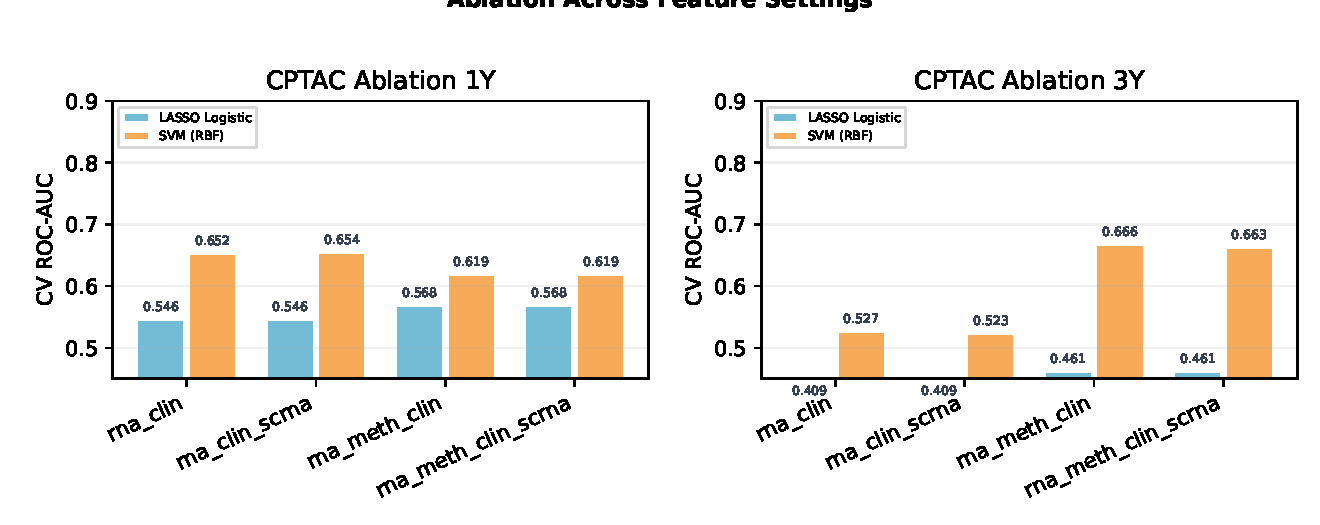
\includegraphics[width=0.88\textwidth]{figures/fig_v7_ablation_auc.pdf}
\caption{CPTAC internal ablation across four feature settings. Methylation provides the strongest incremental signal, especially for 3-year survival, whereas the current six scRNA-derived program scores induce only small changes.}
\label{fig:v7_ablation}
\end{figure*}

\subsection{External Risk Stratification}

To test whether the best external model also separates overall survival trajectories, we converted the best 3-year model (LASSO logistic) into median-split high- and low-risk TCGA groups. Fig.~\ref{fig:v7_external_km} shows a visible but non-significant separation trend (log-rank $p=0.186$). This non-significant result is important: it confirms that the strict external setting is materially harder than pooled cross-validation and motivates further improvement in covariate coverage and cohort size before claiming clinically robust risk stratification.

\begin{figure}[t]
\centering
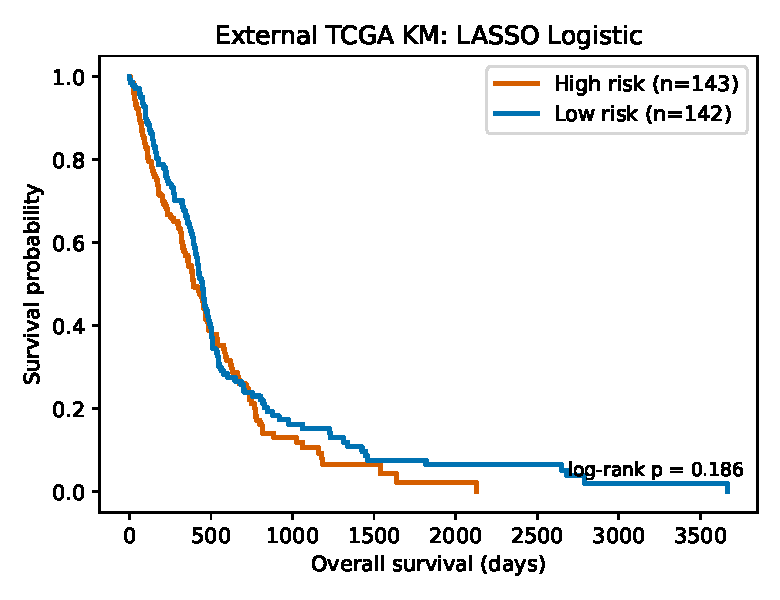
\includegraphics[width=0.48\textwidth]{figures/fig_v7_external_kaplan_meier}
\caption{External TCGA Kaplan--Meier curves using the best 3-year external model (LASSO logistic). Median-split risk groups show a survival trend, but the separation is not yet statistically significant.}
\label{fig:v7_external_km}
\end{figure}
